\section{Chọn bộ truyền đai}
\subsection{Chọn loại đai}
Dựa vào công suất động cơ là $P_{dc} = 4.275 kW$ và số vòng quay $n_{dc} = 950$ vòng/phút và hình 4.1 tài liệu [1]\\
$\Rightarrow$ Chọn đai loại C \\
\begin{figure}[H]
    \centering
    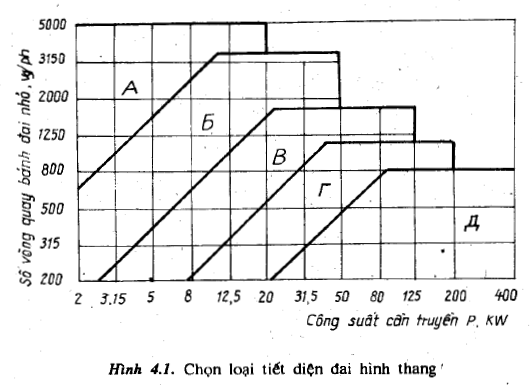
\includegraphics[width=0.5\textwidth]{pictures/chonloaidai.png}
\end{figure}

\subsection{Tính đường kính bánh đai nhỏ}
Theo dãy giá trị tiêu chuẩn tài liệu [1], ta chọn $d_1 = 280 (mm)$.\\
Vận tốc dài trên bánh đai nhỏ:\\
\[
    v_1 = \frac{\pi d_1 n_1}{60000} = \frac{\pi \cdot 280 \cdot 950}{60000} = 13.928 (m/s) < 25 (m/s)
\]  
$\Rightarrow$ Thỏa điều kiện $v_1$ < 25 (m/s) \\
\subsection{Chọn hệ số trượt tương đối và tính đường kính bánh đai lớn}
Chọn hệ số trượt tương đối $\xi = 0.02$ \\
Từ công thức tỉ số của bộ truyền đai: \\
\[
    u_d = \frac{d_2}{d_1(1 - \xi)}
\]s
\[
    \Rightarrow d_2 = u_d \cdot d_1(1 - \xi) = 2.665 \cdot 280(1 - 0,02) = 761.428 (mm)
\]
Theo bảng 4.21 tài liệu [1], ta chọn $d_2 = 710 (mm)$
\begin{figure}[H]
    \centering
    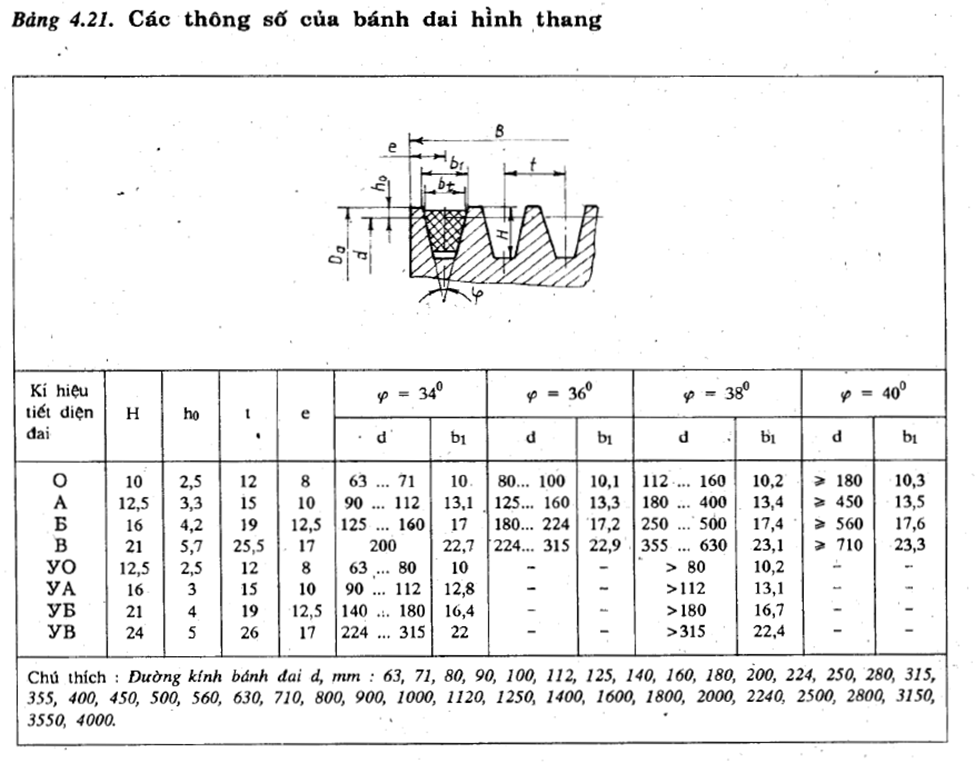
\includegraphics[width=1\textwidth]{pictures/bang4.21.png}
\end{figure}
Tính lại tỷ số truyền:
\[
    u_d = \frac{d_2}{d_1(1 - \xi)} = \frac{710}{280 \cdot 0,98} = 2.587
\]
Tính sai lệch của tỷ số truyền:
\[
    \Delta u = \frac{2.665 - 2.587}{2.665} \cdot 100\% = 2,92\%
\]
$\Rightarrow$ Sai lệch của tỷ số truyền nằm trong phạm vi cho phép.

\subsection{Tính khoảng cách trục a và chiều dài đai L}
\begin{figure}[H]
    \centering
    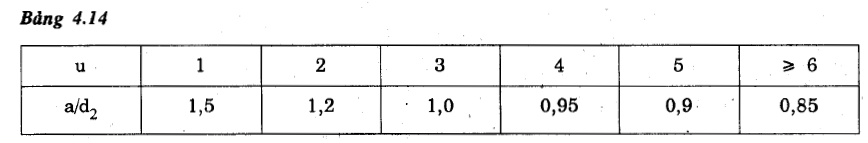
\includegraphics[width=1\textwidth]{pictures/bang4.14.png}
\end{figure}
Dựa vào bảng 4.14 tài liệu [1], ta chọn $a = d_2 = 710 (mm)$ \\
Kiểm tra điều kiện:
\[
    0.55(d_1 + d_2) + h \leq a \leq 2(d_1 + d_2)
\]
\[
    0.55(280 + 710) + 10.5 \leq 710 \leq 2(280 + 710)
\]
\[
    555 \leq 710 \leq 1980 
\]
$\Rightarrow$ Chọn a = 710 (mm) thỏa điều kiện. \\
Chiều dài đai: \\
\[
    L = 2a + \pi\frac{(d_1 + d_2)}{2} + \frac{(d_2 - d_1)^2}{4a} = 2 \cdot 710 + \pi\frac{(280 + 710)}{2} + \frac{(710 - 280)^2}{4 \cdot 710} =  3040.2(mm)
\]
$\Rightarrow$ Chọn chiều dài đai L = 3150 mm theo bảng 4.13. \\
\begin{figure}[H]
    \centering
    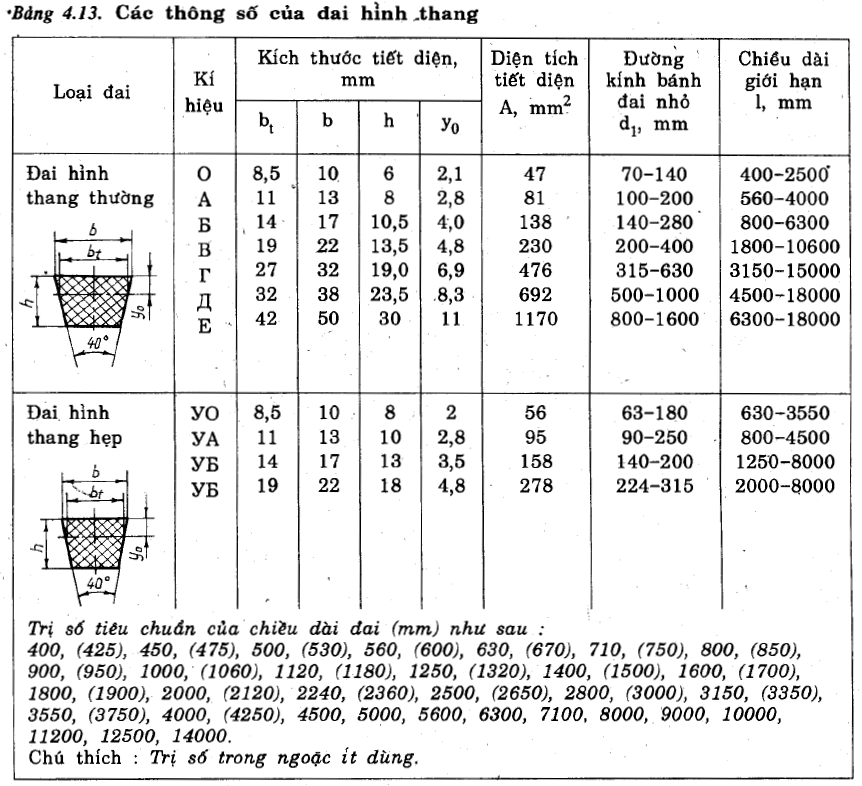
\includegraphics[width=1\textwidth]{pictures/bang4.13.png}
\end{figure}
Kiểm nghiệm đai về tuổi thọ
\[
    i = \frac{v}{L} = \frac{13.928}{3.150} = 4.42/s < i_{max} = 10/s
\]
Tính lại khoảng cách trục: 
\[
    a = \frac{\lambda + \sqrt{\lambda^2 - 8\Delta^2}}{4} = \frac{1594.911 + \sqrt{1594.911^2 - 8 \cdot 215^2}}{4} = 767 (mm)
\]
Trong đó:
\begin{itemize}
    \item $\lambda = L - \frac{\pi(d_1 + d_2)}{2} = 3150 - \frac{\pi(280+710)}{2} = 1594.911$ 
    \item $\Delta = \frac{d_2-d_1}{2} = \frac{710-280}{2} = 215$
\end{itemize}

\subsection{Tính góc ôm đai}
\[
    \alpha_1 = 180 - 57\frac{d_2 - d_1}{a} = 180 - 57\frac{710 - 280}{767} = 148^{\circ} > a_{min} = 120^{\circ}
\]

\subsection{Xác định số đai}
Số đai z được tính theo công thức: 
\[
    z = \frac{P_1K_d}{[P_0]C_\alpha C_L C_u C_z}
\]
\[
    = \frac{4.275 \cdot 1.25}{3.52 \cdot 0.92 \cdot 1.07 \cdot 1.136 \cdot 1} = 1.36
\]
Trong đó:
\begin{itemize}
    \item $P_1 = 4.275 (kW)$ - công suất trên trục bánh dẫn
    \item $K_d = 1.25$ - hệ số tải trọng động
    \item $[P_0] = 3.52 (kW)$ - trị số công suất cho phép (bảng 4.19)
    \item $C_\alpha = 0.92$ - hệ số ảnh hưởng góc ôm đai (bảng 4.15)
    \item $C_L = 1.07$ - hệ số ảnh hưởng chiều dài đai (bảng 4.16)
    \item $C_u = 1.136$ - hệ số ảnh hưởng của tỉ số truyền (bảng 4.17)
    \item $C_z = 1$ - hệ số ảnh hưởng sự phân bố không đều tải trọng các dây đai (bảng 4.18)
\end{itemize}   
Lấy z = 1 đai. \\

\subsection{Chiều rộng bánh đai}
\[
    B = (z - 1)t +2e = (1 - 1)19 + 2 \cdot 12.5 = 37.5 (mm)
\]
Với:
\begin{itemize}
    \item e = 12.5 
    \item t = 19
\end{itemize}

\subsection{Đường kính ngoài của bánh đai}
\[
    d_a = d + 2h_0 = 280 + 2 \cdot 4.2 = 288.4 (mm)
\]
Trong đó $h_0$ = 4.2 (mm). \\

\subsection{Xác định lực căng ban đầu và lực tác dụng lên trục}
Lực căng trên mỗi dây đai:
\[
    F_0 = \frac{780P_1K_d}{vC_\alpha z} + F_v 
\]
\[
    = \frac{780 \cdot 4.275 \cdot 1.25}{13.928 \cdot 0.92 \cdot 1} + 34.53 =  359.815 (N)
\]
Trong đó:
\begin{itemize}
    \item $F_v = q_mv^2 = 0.178 \cdot 13.928^2 = 34.53$ N
    \item $q_m = 0.178$ kg/m
    \item $K_d = 1.25$
    \item $P_1 = 4.275$ kW
    \item $v = 13.928$ m/s
    \item $C_\alpha = 0.92$ 
    \item $z = 1$
\end{itemize}
Lực tác dụng lên trục 
\[
    F_r = 2F_0zsin(\frac{\alpha_1}{2})
\]
\[
    = 2 \cdot 359.815 \cdot 1 \cdot sin(\frac{148}{2}) =  691,753 (N)
\]
\cleardoublepage